\chapter{プロトタイプの実装}
\label{chap:prototype}

この章では本研究でのプロトタイプを実装し、その流れを解説する。

\section{実装概要}
大量のデータをやりとりすることを想定してnode.js\footnote{http://www.nodejs.org/}で実装した。またデータベースはmongoDB\footnote{http://www.mongodb.org/}を採用し、軽量フレームワークを実現した。元になっているセンサーデータはLindaを利用し、データを取得、書き込みしている。

クライアントサイドではJQuery UI\footnote{http://jqueryui.com/}とSVG\footnote{http://www.w3.org/Graphics/SVG/}を使い、ドラッグ&ドロップと線の描画を実現している。

\section{ページ遷移}
パスによってページを管理している。基本的にはパスの名前が最終的に結びつけるオブジェクトの名前になっている。パスにアクセスした際、オブジェクトが作成されていなかった場合には新しいオブジェクトの作成が促され、データベースに記録される。ユーザーはそのオブジェクトに対してアクションとその条件を指定することでプログラムしていく。/keyというページに最初にアクセスした際にはkeyオブジェクトを作成する。最終的なアクションは/key/outputでPOST送信先を設定する。例えば部屋の明るさをセンシングし、部屋が暗くなったらという条件をkeyオブジェクトに紐付け、携帯に通知を送るというアクションを実行することなどができる。その他にも鍵の開け閉めをWebで管理している場合にはそのURLにリクエストを送ることもできる。

/controlのパスはデータベースの管理ができるようになっており、センサーやオブジェクトに追加が出来るようになっている。


\section{サーバーサイド}
言語はJavascriptを使い、node.jsのsocket.io\footnote{http://socket.io/}で実装した。センサーオブジェクトに対して常にコネクションを貼り、データをemitしている。mongoDBではセンサーデータ、オブジェクトデータ、コネクションデータ、クライアントデータを保存している。

\section{クライアントサイド}
クライアントサイドもサーバーサイドと同様にJavascriptを選択した。ページ内でオブジェクトの作成、移動、コネクションの作成などのアクションが行われた際に常にサーバー側に情報を送り保存している。イベントの制御にはEvent Emitter\footnote{http://nodejs.org/api/events.html}を用いた。Event Emitterを使えばオブジェクト自体にイベントを持たせることができる。それぞれのオブジェクトが送られてきたデータを監視し、自分の持っている条件にマッチしたら自らが送信側になるという実装をしている。下の図ではdelta/sensor/lightというセンサーを親データとして、orというオブジェクトが監視して条件に照らし合わせマッチしたら発信するオブジェクトになっている。(図\ref{fig:image09})

\begin{figure}[htbp]
  \begin{center}
    \fbox{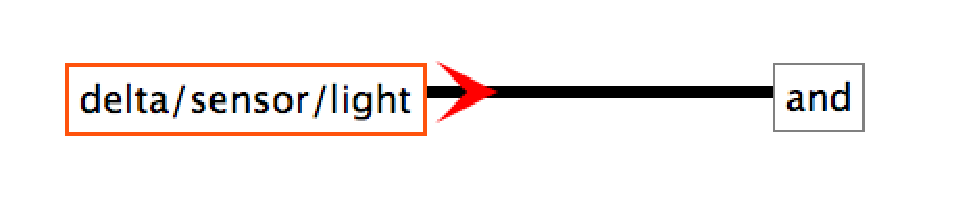
\includegraphics[width=100mm]{image/image09.eps}}
  \end{center}
  \caption{センサーデータの親子関係}
  \label{fig:image09}
\end{figure}

